\documentclass[]{elsarticle} %review=doublespace preprint=single 5p=2 column
%%% Begin My package additions %%%%%%%%%%%%%%%%%%%
\usepackage[hyphens]{url}

  \journal{the 2020 SER Meeting} % Sets Journal name


\usepackage{lineno} % add
\providecommand{\tightlist}{%
  \setlength{\itemsep}{0pt}\setlength{\parskip}{0pt}}

\usepackage{graphicx}
\usepackage{booktabs} % book-quality tables
%%%%%%%%%%%%%%%% end my additions to header

\usepackage[T1]{fontenc}
\usepackage{lmodern}
\usepackage{amssymb,amsmath}
\usepackage{ifxetex,ifluatex}
\usepackage{fixltx2e} % provides \textsubscript
% use upquote if available, for straight quotes in verbatim environments
\IfFileExists{upquote.sty}{\usepackage{upquote}}{}
\ifnum 0\ifxetex 1\fi\ifluatex 1\fi=0 % if pdftex
  \usepackage[utf8]{inputenc}
\else % if luatex or xelatex
  \usepackage{fontspec}
  \ifxetex
    \usepackage{xltxtra,xunicode}
  \fi
  \defaultfontfeatures{Mapping=tex-text,Scale=MatchLowercase}
  \newcommand{\euro}{€}
\fi
% use microtype if available
\IfFileExists{microtype.sty}{\usepackage{microtype}}{}
\bibliographystyle{elsarticle-harv}
\usepackage{graphicx}
% We will generate all images so they have a width \maxwidth. This means
% that they will get their normal width if they fit onto the page, but
% are scaled down if they would overflow the margins.
\makeatletter
\def\maxwidth{\ifdim\Gin@nat@width>\linewidth\linewidth
\else\Gin@nat@width\fi}
\makeatother
\let\Oldincludegraphics\includegraphics
\renewcommand{\includegraphics}[1]{\Oldincludegraphics[width=\maxwidth]{#1}}
\ifxetex
  \usepackage[setpagesize=false, % page size defined by xetex
              unicode=false, % unicode breaks when used with xetex
              xetex]{hyperref}
\else
  \usepackage[unicode=true]{hyperref}
\fi
\hypersetup{breaklinks=true,
            bookmarks=true,
            pdfauthor={},
            pdftitle={2020 SER Meeting Abstract},
            colorlinks=false,
            urlcolor=blue,
            linkcolor=magenta,
            pdfborder={0 0 0}}
\urlstyle{same}  % don't use monospace font for urls

\setcounter{secnumdepth}{0}
% Pandoc toggle for numbering sections (defaults to be off)
\setcounter{secnumdepth}{0}


% Pandoc header



\begin{document}
\begin{frontmatter}

  \title{2020 SER Meeting Abstract}
    \author[biostat-berkeley]{Nima S. Hejazi}
  
    \author[epibiostat-berkeley]{Mark J. van der Laan}
  
    \author[fredhutch]{Holly E. Janes}
  
    \author[fredhutch]{Peter B. Gilbert}
  
    \author[emory]{David C. Benkeser}
  
      \address[biostat-berkeley]{Graduate Group in Biostatistics, University of California, Berkeley}
    \address[epibiostat-berkeley]{Division of Epidemiology and Biostatistics, University of California,
Berkeley}
    \address[fredhutch]{Vaccine and Infectious Disease Division, Fred Hutchinson Cancer Research
Center}
    \address[emory]{Department of Biostatistics and Bioinformatics, Emory University}
      \cortext[1]{Character count: 1990 (with spaces)}
    \cortext[2]{Corresponding author: nhejazi@berkeley.edu}
    \cortext[3]{Key words: causal inference, two-phase sampling, stochastic
intervention, targeted learning, vaccine efficacy}
    \cortext[4]{Title: Assessing the causal effects of stochastic interventions in
vaccine efficacy trials with two-phased designs}
  
  \begin{abstract}
  
  \end{abstract}
  
 \end{frontmatter}

Causal inference has traditionally focused on the effects of static
interventions, under which the magnitude of the treatment is set to a
fixed, prespecified value for each unit. The evaluation of such
interventions faces a host of issues, among them non-identification,
violations of the assumption of positivity, and inefficiency. Stochastic
interventions provide a promising solution to these fundamental issues
by allowing for the target parameter to be defined as the mean
counterfactual outcome under a hypothetically shifted version of the
observed exposure distribution. Despite the promise of such approaches,
real data analyses are often further complicated by economic
constraints, such as when the primary variable of interest is far more
expensive to collect than auxiliary covariates. Two-phase sampling
schemes are often used to bypass such limitations -- unfortunately,
their use produces side effects that require further adjustment when
formal statistical inference is the principal goal of a study. We
present a novel approach for use in such settings: augmented targeted
minimum loss and one-step estimators for the causal effects of
stochastic interventions, with guarantees of consistency, efficiency,
and multiple robustness even in the presence of two-phase sampling. We
further propose a technique that utilizes the estimated causal effects
of stochastic interventions to construct a nonparametric working
marginal structural model to summarize the effect of shifting an
exposure variable on the outcome of interest, analogous to a
dose-response analysis. Using data from the recent HVTN 505 HIV vaccine
efficacy trial, we demonstrate this technique by assessing the effects
of changes in post-vaccination immunogenicity on HIV-1 acquisition
across a range of possible shifts, outlining a highly interpretable
variable importance measure for ranking multiple immune responses based
on their utility as immunogenicity study endpoints in future HIV-1
vaccine trials.

\newpage

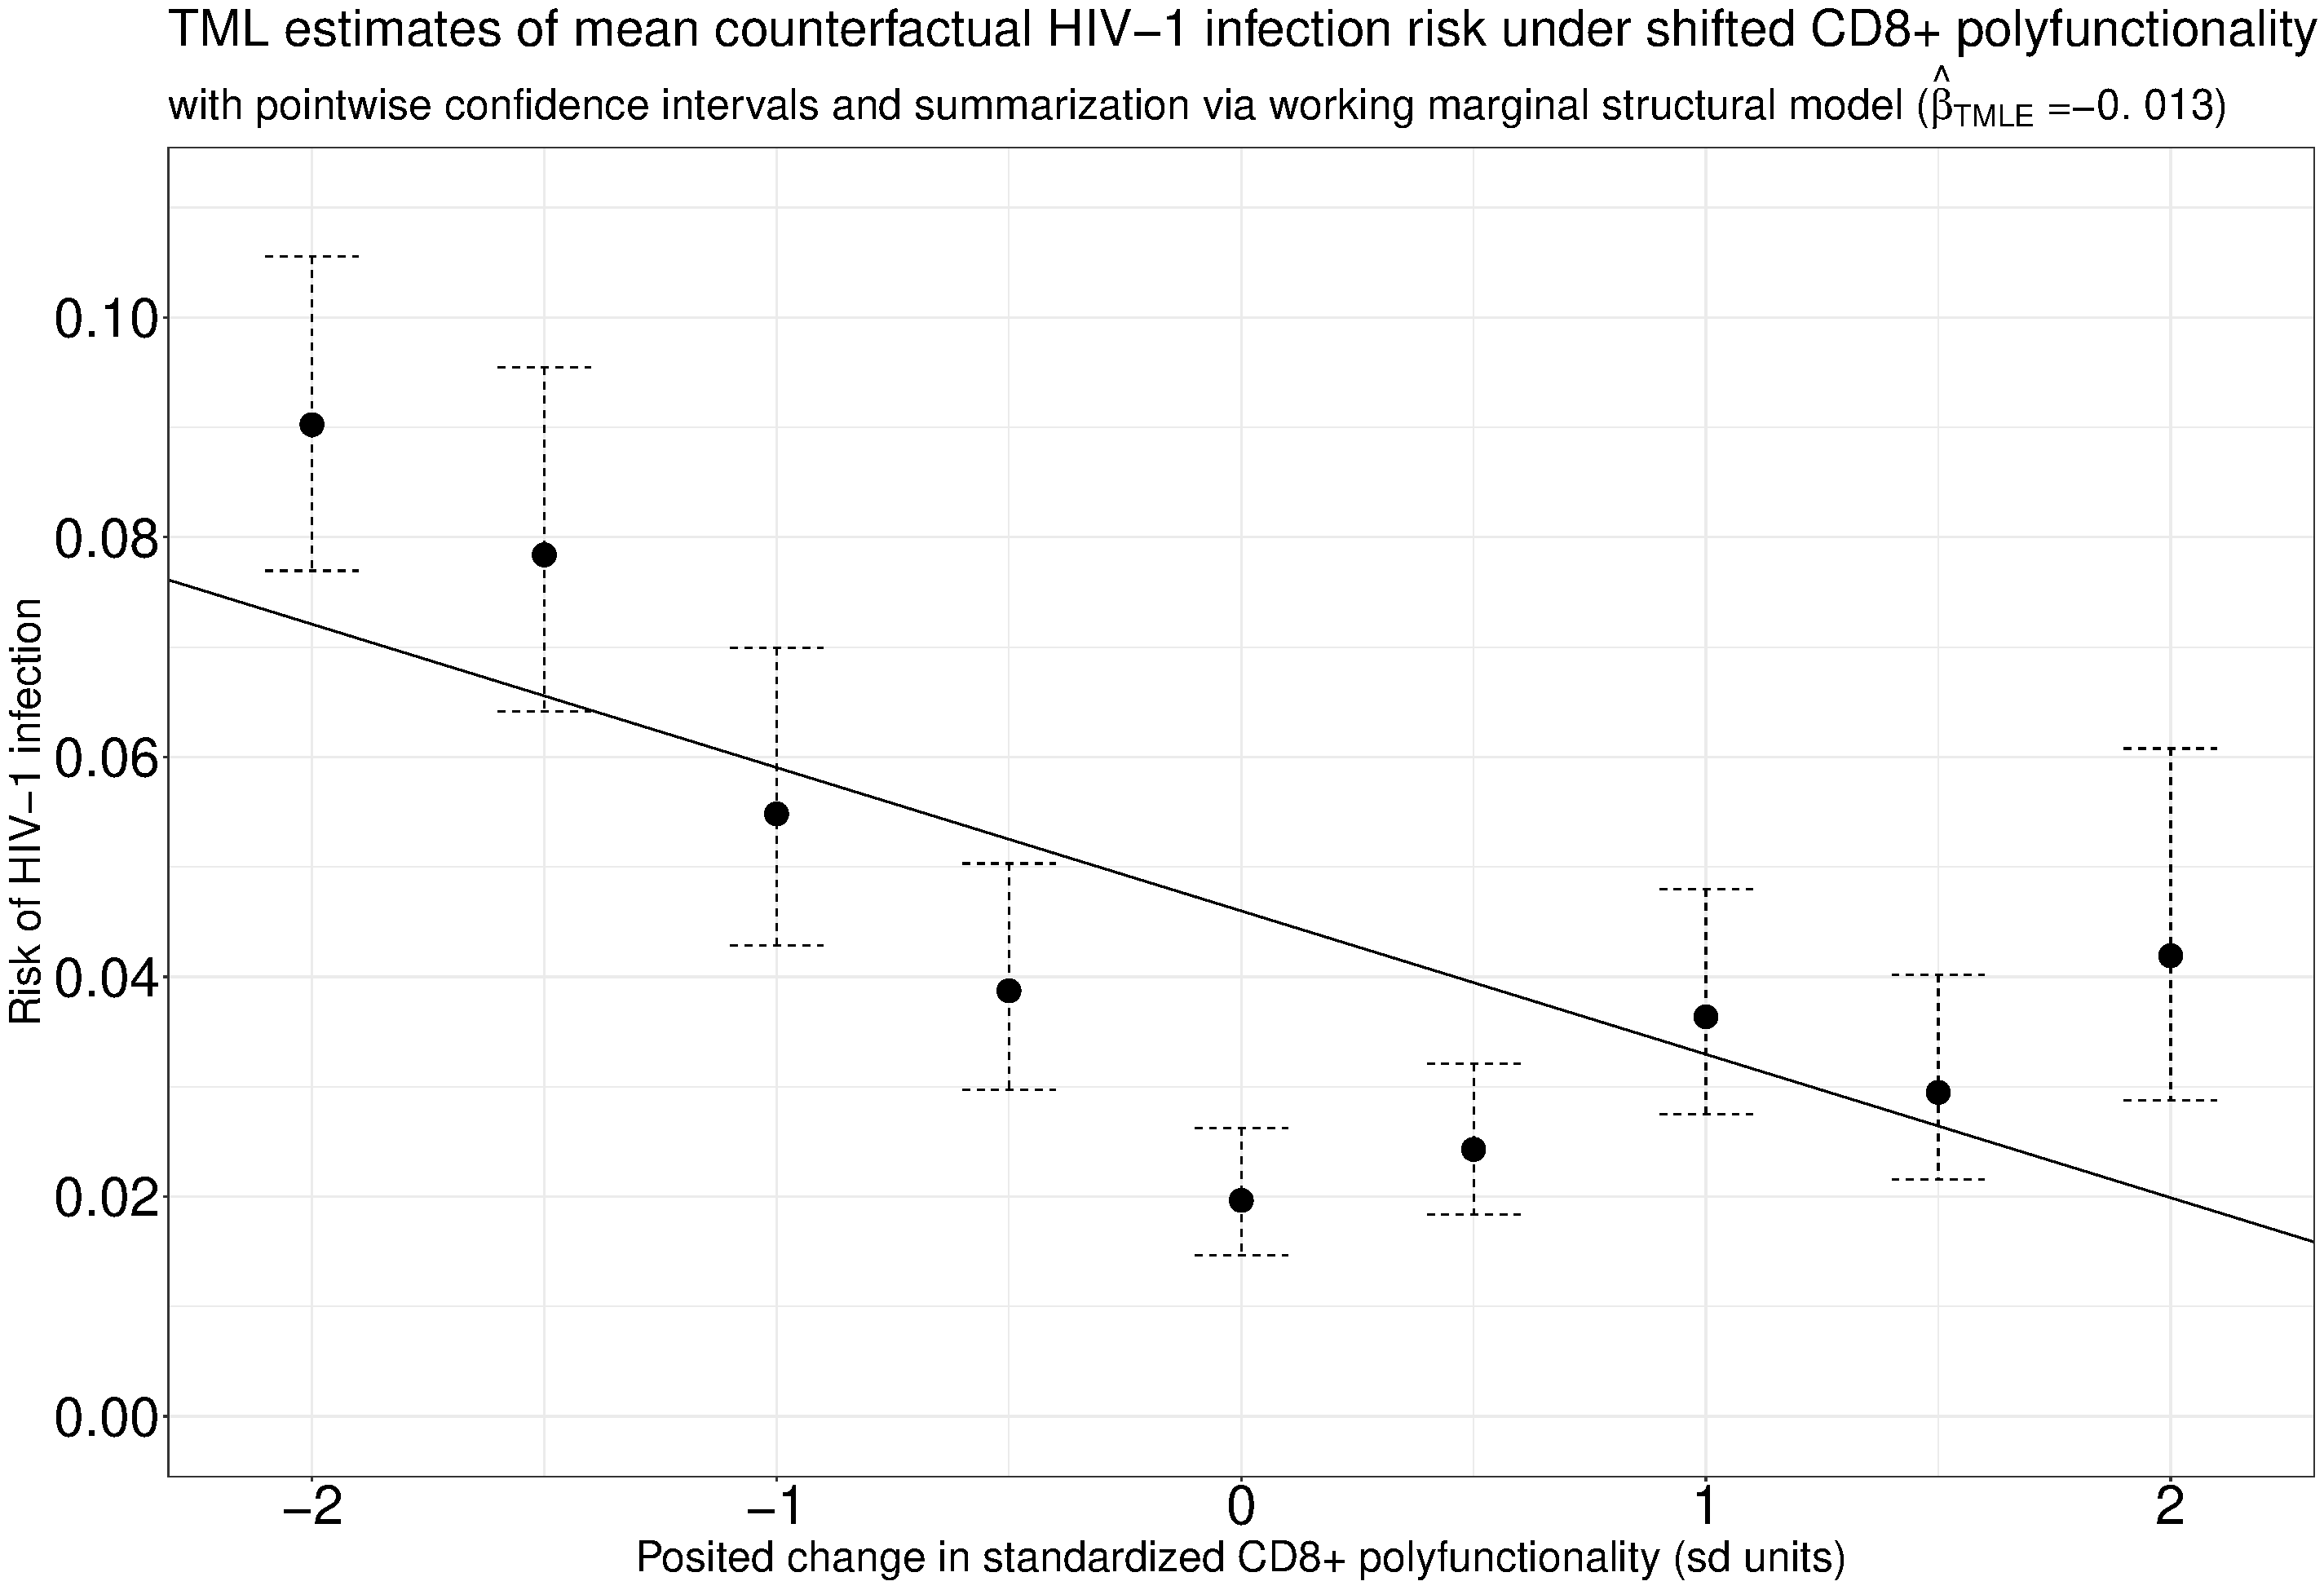
\includegraphics{./cd8_msm_tmle_summary.pdf}


\end{document}


